\documentclass[11pt]{article}

\usepackage{acl2014}
\usepackage{times}
\usepackage{latexsym}
\usepackage{amsmath}
\usepackage{amssymb}
\usepackage{graphicx}
\usepackage{multicol}
\usepackage{url}

\newcommand{\Eq}[1]{Equation (\ref{eq:#1})}
\newcommand{\eq}[1]{Equation (\ref{eq:#1})}
\newcommand{\eqlabel}[1]{\label{eq:#1}}
\newcommand{\Fig}[1]{Figure~\ref{fig:#1}}
\newcommand{\fig}[1]{Figure~\ref{fig:#1}}
\newcommand{\figlabel}[1]{\label{fig:#1}}

\newcommand{\etal}{\emph{et al.}}

\DeclareMathOperator*{\argmax}{arg\,max}
\DeclareMathOperator*{\argmin}{arg\,min}

\title{Collaborative Topic Modeling Applied to the \emph{ArXiv}}

\author{Daniel Foreman-Mackey \\ {\tt danfm@nyu.edu} \\}

\begin{document}
\maketitle

\begin{abstract}
In this paper, I implement a recommendation engine based on the collaborative
topic model developed by Wang \& Blei~\shortcite{ctr} and use it to recommend
scientific articles published on the \emph{ArXiv}.
This model avoids the ``cold start'' problem that plagues traditional
collaborative filtering approaches by training a latent representation based
on a topic model trained on the full ArXiv corpus.
I evaluate the performance of this model and compare it to several competing
recommendation algorithms by computing the recall of the recommendations on
user bibliographies from the CiteULike service.
On this dataset, a purely collaborative algorithm marginally outperforms the
collaborative topic model when recommending articles that appear in at least
five user bibliographies.
For new articles that are not included in the training bibliographies, the
collaborative topic model offers excellent recommendations and far outperforms
a simple tf--idf based cosine distance metric.

The code is available on GitHub at \url{https://github.com/dfm/clda} under
the terms of the MIT License.
\end{abstract}

\section{Introduction}

With a huge number of scientific articles published every day, it can be
difficult to discover relevant papers from the literature and keep up with
recent results.
There are services that recommend personalized lists of similar articles
(such as Google Scholar\footnote{\url{http://scholar.google.com}},
Mendeley\footnote{\url{http://www.mendeley.com}}, and
PubMed\footnote{\url{http://www.ncbi.nlm.nih.gov/pubmed}}) but these systems
all use some combination of collaborative filtering, tags, and hand curation.
As a result, the recommendations aren't terribly robust for new articles.

An interesting place to make progress on this problem is the astrophysics
literature because the full-text and a set of metadata for almost every paper
published in the past 20 years is publicly available on the
\emph{ArXiv}\footnote{\url{http://arxiv.org}}.
There are also 50--100 articles posted daily to the ArXiv's \emph{astro-ph}
category and about the same number again in computer science.

In this paper, I describe and implement a collaborative topic model based on
Wang \& Blei~\shortcite{ctr}.
Using this model, I test the recommendation quality using user bibliographies
from CiteULike\footnote{\url{http://www.citeulike.org}} and compare the
results to some standard recommendation models.
The collaborative topic model provides competitive recommendations of both old
articles from the literature and newly published articles.

\section{Recommendation by collaborative filtering}

A very successful class of recommendation techniques is called
\emph{collaborative filtering}.
This problem is generally cast as a matrix factorization model where users and
documents are described by latent vectors---$\mathbf{u}_i$ and $\mathbf{v}_j$
respectively---of some dimension $K$ and the predicted rating (by user $i$ of
document $j$) is
\begin{eqnarray}
r_{ij} &=& \mathbf{u}_i^\mathrm{T} \, \mathbf{v}_j + \mathrm{noise} \quad.
\end{eqnarray}
The full $N_\mathrm{users}\times N_\mathrm{docs}$ matrix of ratings is then
\begin{eqnarray}
R &=& U^\mathrm{T}\,V + \mathrm{noise}
\end{eqnarray}
where $U$ and $V$ are the matrices of user and item vectors.
The matrix $R$ is generally extremely sparse ($\sim 99.8\%$ in this specific
case) and the meaning of the unobserved entries is somewhat ambiguous and
shouldn't always be considered negative ratings.

To make matters worse, in case of scientific article recommendation, let's
assume that we don't have explicit feedback like starred ratings.
Instead, we have only implicit feedback: is the article in the bibliography or
not?
To approach this problem, I implemented the \emph{implicit feedback
collaborative filtering} (ICF) algorithm described by Hu, Koren
\& Volinsky~\shortcite{icf}.
The main idea behind this algorithm is that they treat the null entries in the
$R$ matrix as low-confidence negative ratings and the observed entries
as higher-confidence positive indicators.
Then, they perform the full probabilistic matrix factorization on this system.
Specifically, the log-likelihood function is
\begin{eqnarray}\label{eq:lnlike}
\mathcal{L} &=& -\sum_{i,j}
                c_{ij}\,(r_{ij}-\mathbf{u}_i^\mathrm{T}\,\mathbf{v}_j)^2
\nonumber\\
&& - \lambda_u\,\sum_i \mathbf{u}_i^\mathrm{T}\,\mathbf{u}_i
 - \lambda_v\,\sum_j \mathbf{v}_j^\mathrm{T}\,\mathbf{v}_j
\end{eqnarray}
where $c_{ij}$ is the model's confidence in the rating $r_{ij}$.
In this particular context, our model will have $r_{ij} = 1$ if document $j$
is in user $i$'s library and $r_{ij} = 0$ otherwise.

The maximum likelihood result for equation~\ref{eq:lnlike} is \cite{icf}
\begin{eqnarray}\eqlabel{icf-update}
\mathbf{u}_i &\gets& (V\,C_i\,V^\mathrm{T}+\lambda_u)^{-1}\,
                     V\,C_i\,\mathbf{r}_i
\quad \mathrm{and} \nonumber \\
\mathbf{v}_j &\gets& (U\,C_j\,U^\mathrm{T} + \lambda_v)^{-1}\,U\,C_j\,
                     \mathbf{r}_j
\end{eqnarray}
where $C_{i/j}$ is the diagonal matrix of confidences and $\mathbf{r}_{i/j}$
is the vector of ratings for user $i$/document $j$.
In practice, I iterate between updating the user and document vectors until
convergence.
Due to the structure of the model, the computational cost associated with each
update scales linearly with the number of ratings in the dataset \cite{icf}.

I chose to use the same confidence model as Hu \etal~(2008)
\begin{eqnarray}
c_{ij} &=& 1+\alpha\,r_{ij}
\end{eqnarray}
where $\alpha$ is a free parameter.

A major shortcoming of a simple collaborative filtering model like this is
that it cannot compute scores for documents or users that are not in the
training data.
As a result, this vanilla implementation provides no robust technique for
personalized recommendation of recent articles.
Below, I'll describe a generalization of this model that uses a topic
representation of the latent dimension in order to avoid this problem.

\section{Topic modeling with LDA}

Latent Dirichlet Allocation (LDA) is a popular topic model where a document
$d$ in a corpus is represented as a mixture of topics $\theta_d$ \cite{lda}.
The latent per-word topics $z_{dn}$ are then drawn from this mixture.
LDA is popular because it has been shown to uncover qualitative structure in
corpora.
There have also been efficient variational inference and online learning
algorithms developed \cite{ovlda}.

For this project, I implemented the \emph{online variational} learning
algorithm as described by Hoffman \etal~(2010).
These authors also released a Python implementation of this algorithm---under
the GPLv3 license---but I independently implemented my own version with a more
user-friendly API, a more liberal license (MIT), and built-in parallelization.

This algorithm has about a dozen tunable parameters (learning rate, vocabulary
size, number of topics, mini-batch size, hyperparameters, \emph{etc.}) and I
didn't have the time or resources to systematically tune them all using cross
validation.
That being said, I did spend some time exploring the effects of some of the
parameters.
For example, \fig{lda-results} shows an estimate of the perplexity computed on
a held-out validation set of 1024 documents from the ArXiv for different model
complexities.
The details of this dataset are described below.
For each curve in the figure, the entire corpus was only passed through
approximately twice but it seems to have converged.

The fact that even a 300 topic model performs well on the held-out set
suggests that I'm not over-fitting the training data.
This is not surprising given the broad set of subjects that are published on
the ArXiv and I'll argue below that 300 topics might not be fine enough for
our purpose.

The key feature of this model for our purposes here is that it provides a
latent representation of a document---$\theta_d$ above---based only on its
contents.
If we train our collaborative filtering model properly, we should be able to
use this representation to give reasonable recommendations for new articles.
This is the intuition that I'll discuss in the next section.

\begin{figure}
\centering
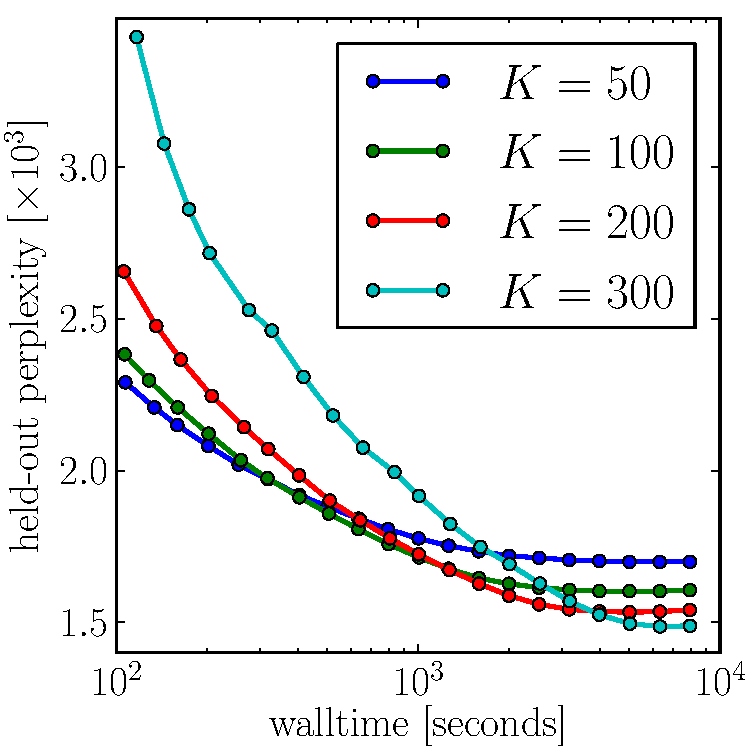
\includegraphics[width=0.4\textwidth]{lda-results-k.pdf}
\caption{%
The held-out perplexity as a function of runtime for different model
topic model complexities.
The model is trained on all of the abstracts and titles in the ArXiv database
except 1024 randomly chosen articles that are used to compute the perplexity.
The full corpus is passed through the training process approximately twice for
each model.
\figlabel{lda-results}}
\end{figure}

\section{Collaborative LDA}

Wang \& Blei~(2011) proposed a collaborative generalization of LDA (CLDA) that
includes user data.
The graphical model for CLDA is shown in \fig{clda} and the top row of the
model is just the familiar LDA model and the bottom row shows the regularized
matrix factorization model.
The generative story for this model is
\begin{itemize}
\item{the documents---and, in particular, the topic fractions $\theta_d \sim
\mathrm{Dir}(\alpha)$---are generated as they would be in LDA,}
\item{the latent document representation $\mathbf{v}_d \gets \theta_d +
\epsilon_d$ where the \emph{topic offset} $\epsilon_d$ is drawn from the
zero-centered normal $\mathcal{N} (\mathbf{0},\lambda_v)$,}
\item{the latent user representation $\mathbf{u}_i$ is drawn from the normal
$\mathcal{N}(\mathbf{0},\lambda_u)$, and}
\item{the implicit rating is generated---as it is in ICF---from a normal with
precision $c_{id}$,
$\mathcal{N}(\mathbf{u}_i^\mathrm{T}\,\mathbf{v}_d,c_{id})$.}
\end{itemize}

For fixed $\theta_d$, the matrix factorization updates differ from
\eq{icf-update} by one term \cite{ctr}
\begin{eqnarray}\eqlabel{clda-update}
\mathbf{u}_i &\gets& (V\,C_i\,V^\mathrm{T}+\lambda_u)^{-1}\,
                     V\,C_i\,\mathbf{r}_i
\quad \mathrm{and} \\
\mathbf{v}_d &\gets& (U\,C_d\,U^\mathrm{T} + \lambda_v)^{-1}\,(U\,C_d\,
                     \mathbf{r}_d + \lambda_v\,\theta_d) \quad \nonumber
\end{eqnarray}
and can still be computed in linear time.
Wang \& Blei~\shortcite{ctr} proposed a heuristic learning algorithm to
simultaneously infer the latent CF variables and the LDA topic proportions but
found that the results were identical when they trained the LDA model
independently and then held the topic mixtures fixed.
Their algorithm also requires full batch updates of the LDA parameters
yielding it computationally intractable on large datasets like the one I'm
using here.
In the experiments described in the following section, I'll use a pre-trained
LDA model and only train the $\mathbf{u}_i$ and $\epsilon_d$ parameters on the
CF data, assuming fixed $\theta_d$.

\section{Experiments}

\subsection{Datasets}

For these experiments, I'm using the abstracts and titles for every article
published to the ArXiv since the first listing in 1992 until December 10,
2013.
I downloaded these files using the OAI
interface\footnote{\url{http://arxiv.org/help/oa/index}} and tokenized the
data using the NLTK\footnote{\url{http://nltk.org/}} implementation of the
Penn Treebank tokenizer.
These parsed listings are available online at \url{data.arxiv.io} as a SQLite
database\footnote{\url{http://data.arxiv.io/abstracts.db.gz}}.
There are almost 900,000 abstracts in this dataset.

To train the ICF model, I used the user bibliographies from
CiteULike\footnote{\url{http://www.citeulike.org/faq/data.adp}}.
I used a set of regular expressions and
heuristics\footnote{\url{%
https://github.com/dfm/clda/blob/master/scripts/prepare-citeulike-data}} to
extract the links in this dataset corresponding to ArXiv abstracts.
After removing duplicate entries and any user with fewer than 5 items in their
bibliography, we are left with 713 users, 15,688 documents, and 27,189
user-document pairs (99.8\% sparsity).
I extracted a test set of user-items pairs containing 1200 elements
corresponding to articles appearing at least 5 times in the dataset.
This set is constructed in such a way that every document in the test set
appears in the training set at least once and a random number of times in the
test set.

This dataset is not ideal for the problem that I'm trying to solve because the
vast majority of users on CiteULike are computer scientists and biologists
while more than half of the articles on the ArXiv are about astrophysics and
theoretical particle physics.
This means that a topic model trained on the full ArXiv won't necessarily be
the optimal latent representation for many of the articles in the dataset.
Unfortunately, this was the only similar dataset that I could find that was
freely available for academic purposes so it'll have to do.

\subsection{Training the LDA model}

As mentioned previously, I chose to train an LDA model in advance on the full
set of abstracts and titles in the ArXiv dataset.
For the production model, I used 300 topics, a mini-batch size of 4096, and
the hyperparameters $\eta$ and $\alpha$ set to 0.01.
The held-out perplexity curve for this model is shown in \fig{lda-results}.

\subsection{Evaluation}

In general, the performance of a recommendation engine is difficult to assess
without active feedback and there are many different possible metric depending
on your goals.
One particular goal that is hard to evaluate quantitatively is that you might
want to recommend articles (possibly across domains) that the user would not
come across of their own accord.

Since the CiteULike dataset is so sparse and since the null entries are not
necessarily negative ratings, the best evaluation metric is recall on a
held-out dataset.
In particular, I'll consider the recall as a function of the number of
articles recommended.
In practice, at test time, I (hypothetically) recommend the top $N$ articles
to a specific user---chosen from the set of articles that are not in their
training set---and compute the fraction of articles in their test set that
appeared in their list of recommendations.
All of the quoted results are the mean recall across all the users with
articles in the test set.

\subsection{Baseline models}

For comparison, I implemented two baseline models: random and cosine
similarity.
For the random recommendations, I built a ICF model with random $U$ and $V$
vectors and computed the recall using the recommendations generated by this
model.
For the cosine similarity model, I computed the tf--idf representation of each
article and then represented the users as the sum of tf--idf vectors for each
article in their training set.
Then, I ranked the remaining articles using the cosine distance between the
user vector and the article and computed the recall on these recommendations.

\subsection{Results}

The results for the baseline models and my three models are shown in
\fig{results}.
Again, there are many tuning parameters that I was only able to evaluate
superficially but in this figure, I'm showing the following settings:
\begin{itemize}
\item{\emph{LDA} --- for this model, the $V$ matrix is set to the expected
topic distributions inferred using the LDA model and the $U$ matrix is set
with a single pass of \eq{clda-update} on the training set.
This simulates the behavior of the CLDA model on new articles that have never
had reviews.}
\item{\emph{CLDA} --- this is the CLDA model run with 300 topics for 20 full
passes of \eq{clda-update} with $\alpha=1$, $\lambda_v=10$ and $\lambda_u=10$.}
\item{\emph{ICF} --- the ICF model run with 300 topics for 20 passes of
\eq{icf-update} with $\alpha=1$, $\lambda_v=10$ and $\lambda_u=10$.}
\end{itemize}
These parameter settings are by no means optimal but they seemed to be
reasonable choices based on some heuristic experimentation.

\begin{figure}
\centering
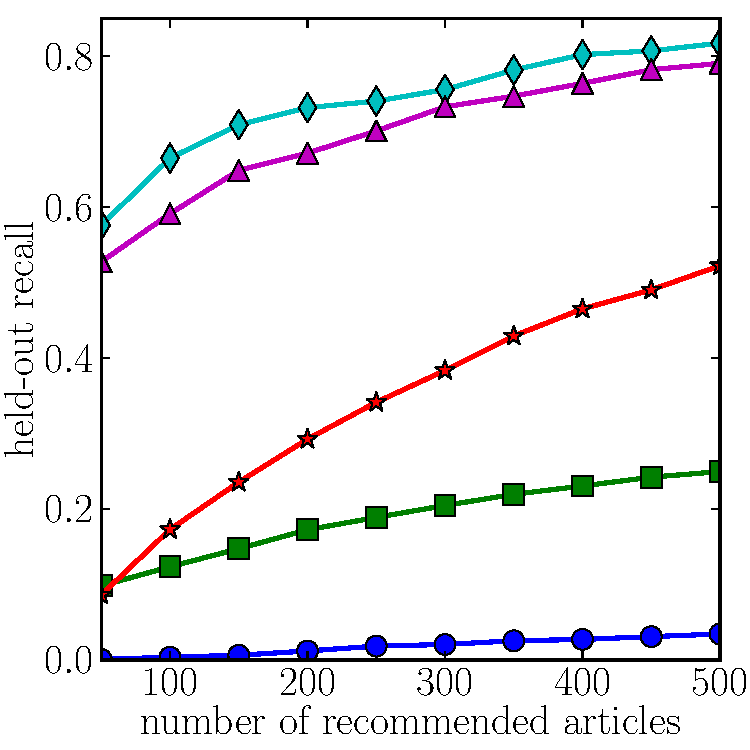
\includegraphics[width=0.4\textwidth]{results.pdf}
\caption{%
The recall curves for the set of tested models.
From worst to best, the models are: random (blue dots), tf--idf (green
squares), LDA (red stars), CLDA (purple triangles), and ICF (cyan diamonds).
See the text for descriptions of these models.
\figlabel{results}}
\end{figure}

\section{Discussion}

These results are somewhat different from the results from Wang \&
Blei~\shortcite{ctr}.
In particular, they found that their CLDA model performed at least as well as
the ICF model in all cases whereas here, I find that ICF out-performs CLDA by
a few percent for in-matrix predictions.
There are a few reasons why this might happen but the most compelling argument
that I can come up with is that the topics determined by CLDA are not
sufficiently fine-grained to represent the documents found in the test set.
This will happen because the topic model is required to put quite a bit of
support in the topic distribution for astrophysics and other topics that are
not well represented in the CiteULike dataset.
Wang \& Blei~\shortcite{ctr} get around this problem by only training their
topic model on the articles in the CiteULike dataset.
This leads to better performance on that dataset but it would generalize to
users in other domains as well.

Despite this particular shortcoming, the CLDA model successfully satisfies the
goals of this project.
The in-matrix recommendations are not substantially worse than a pure
collaborative model and the out-of-matrix recommendations are far better than
the competing tf--idf content based method.
This is a very promising result because I have found that in practice this
tf--idf approach offers qualitatively satisfying suggestions when applied to
the daily listings.

My ultimate goal with this project is to build a web service that offers
personalized daily ArXiv listings and recommendations that highlight a user's
interests.
In this context, the ratings will be constructed with a combination of
explicit (probably binary likes and dislikes) and implicit (clickthroughs,
\emph{etc.}) feedback.
The out-of-matrix CLDA recommendations seem like a good way of going about
building something like this because the recommendation procedure for new
articles is both computationally tractable and horizontally scalable.

\section{Honor Pledge}
I pledge my honor that all the work described in this report is solely mine
and that I have given credit to all third party resources that I have used.

\begin{thebibliography}{}

\bibitem[\protect\citename{Blei, Ng \& Jordan}2003]{lda}
D. Blei, A. Ng, \& M. Jordan.
\newblock{{\bf Latent Dirichlet allocation}}
\newblock{\emph{Journal of Machine Learning Research},}
\newblock{2003.}

\bibitem[\protect\citename{Hoffman, Blei \& Bach}2010]{ovlda}
M. Hoffman, D. Blei, \& F. Bach.
\newblock{{\bf Online learning for latent Dirichlet allocation}}
\newblock{\emph{Neural Information Processing Systems},}
\newblock{2010.}

\bibitem[\protect\citename{Hu, Koren \& Volinsky}2008]{icf}
Y. Hu, Y. Koren, \& C. Volinsky.
\newblock{{\bf  Collaborative filtering for implicit feedback datasets}}
\newblock{\emph{Proceedings of the 2008 Eighth IEEE International Conference
                on Data Mining},}
\newblock{2008.}

\bibitem[\protect\citename{Wang \& Blei}2011]{ctr}
C. Wang \& D. Blei.
\newblock{{\bf Collaborative topic modeling for recommending scientific
           articles}}
\newblock{\emph{Knowledge Discovery and Data Mining},}
\newblock{2011.}

\end{thebibliography}

\begin{multicols}{2}
\begin{figure*}
\centering
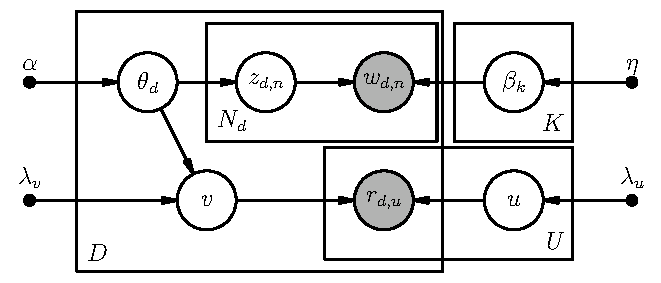
\includegraphics{clda.pdf}
\caption{%
The probabilistic graphical model representation collaborative LDA model.
The top row of nodes is exactly the standard LDA topic model and the bottom is
the graphical model representing the probabilistic matrix factorization model
for collaborative filtering.
\figlabel{clda}}
\end{figure*}
\end{multicols}


\end{document}
